\documentclass[10pt,a4paper,twocolumn]{article}

\usepackage[T1]{fontenc}
\usepackage[utf8]{inputenc}
\usepackage[bahasa]{babel}
\usepackage{newtxtext,newtxmath}
\usepackage[a4paper,top=18mm,bottom=18mm,left=16mm,right=16mm,columnsep=7mm]{geometry}
\usepackage{graphicx}
\usepackage{xcolor}
\usepackage{titlesec}
\usepackage{array}
\usepackage[font=small,labelfont=bf,labelsep=period]{caption}

% Warna judul bagian mengikuti templat dosen; selebihnya hitam.
\definecolor{judulbiru}{HTML}{2F5D9E}
\titleformat{\section}{\color{judulbiru}\large}{\thesection}{1em}{}
\titleformat{\subsection}{\normalsize\bfseries}{\thesubsection}{1em}{}
\titlespacing*{\section}{0pt}{10pt}{5pt}
\titlespacing*{\subsection}{0pt}{8pt}{4pt}

\AtBeginDocument{%
  \renewcommand{\figurename}{Gambar}%
  \renewcommand{\tablename}{Tabel}%
  \renewcommand{\refname}{References / Referensi}%
}

\begin{document}

\twocolumn[{%
\begin{center}
  {\Large\bfseries Computer Vision Final Project: Technical Report\par}
  \vspace{3pt}
  {\large\bfseries Proyek Akhir Visi Komputer: Laporan Teknis\par}
  \vspace{12pt}
  {\large\bfseries Klasifikasi Ordinal Tingkat Kematangan Tandan Buah Segar Kelapa Sawit\\
  dari Foto Lapangan Menggunakan EfficientNet-B0\par}
  \vspace{10pt}
  \begin{tabular}{ll}
    Yedija Teofilus Yonatan & 412024011 \\
    Juanito Dante           & 412024001 \\
    Steven Iwan             & 412024010 \\
  \end{tabular}
\end{center}
\vspace{8pt}
}]

\section*{Abstract}
\noindent\textbf{Abstrak}---Penilaian tingkat kematangan tandan buah segar (TBS) kelapa sawit di pabrik masih dilakukan secara visual oleh petugas sortasi, sehingga hasilnya dapat berbeda antarpetugas. Proyek ini membangun model klasifikasi lima tingkat kematangan (mentah, setengah matang, matang penuh, terlalu matang, dan busuk) dari satu foto. Karena tingkat kematangan bersifat berurutan, kami membandingkan EfficientNet-B0 pra-latih yang dilatih dengan loss \emph{cross-entropy} (CE) dan dengan loss ordinal CORN. Data yang digunakan adalah dataset publik berisi 4.728 foto lapangan dari Kalimantan Tengah. Audit data menunjukkan bahwa foto bernomor berurutan sering memotret tandan yang sama, dan 92\% foto uji pada pembagian data resmi memiliki foto tetangga di data latih. Karena itu, evaluasi utama memakai split blok yang menjaga foto berurutan tetap dalam satu bagian. Pada split blok, kedua model mencapai macro-F1 sekitar 0,91, jauh di atas baseline warna (0,66), tetapi CORN tidak lebih baik daripada CE (macro-F1 0,905 dibanding 0,914; MAE 0,121 dibanding 0,111 tingkat). Pada split resmi, skor kedua model tampak sekitar 5 poin lebih tinggi. Model dijalankan sebagai demo web dengan waktu inferensi sekitar 12~ms per foto pada CPU.

\section{1. Introduction / Pendahuluan}
Indonesia adalah produsen kelapa sawit terbesar di dunia dengan luas areal 16,83 juta hektare, dan menguasai lebih dari 55\% ekspor minyak sawit dunia \cite{pusdatin2024}. Mutu tandan buah segar (TBS) yang dijual pekebun ditentukan terutama oleh tingkat kematangannya. Tandan yang dipanen terlalu dini menghasilkan minyak lebih sedikit, sedangkan tandan yang terlambat dipanen menaikkan kadar asam lemak bebas \cite{woittiez2016}. Di pabrik kelapa sawit, petugas sortasi memeriksa sebagian tandan secara visual lalu memotong berat kiriman bila menemukan tandan mentah \cite{woittiez2016}. Penilaian manual seperti ini bersifat subjektif dan sering memicu sengketa antara pekebun dan pabrik \cite{alfatni2008}.

Pengolahan citra tradisional pernah dipakai untuk masalah ini, misalnya dengan rata-rata nilai RGB, tetapi metode tersebut membutuhkan pencahayaan yang terkontrol \cite{alfatni2008}. Foto di kebun diambil dengan ponsel yang berbeda, di bawah terik atau teduh, dan dengan latar yang beragam. Kematangan juga tidak hanya terlihat dari warna, tetapi juga dari tekstur buah, buah yang mulai rontok, dan kekeringan tandan (Gambar~\ref{fig:kelas}). \emph{Convolutional neural network} (CNN) dapat mempelajari isyarat tersebut langsung dari contoh foto \cite{suharjito2021}, dan dengan \emph{transfer learning} dari ImageNet \cite{deng2009}, CNN dapat dilatih dengan beberapa ribu foto saja.

Kelima tingkat kematangan bersifat berurutan. Salah menilai tandan mentah sebagai setengah matang lebih ringan akibatnya daripada menilainya sebagai terlalu matang. Dataset yang kami gunakan memang disusun sebagai data ordinal \cite{kamal2024}, tetapi loss \emph{cross-entropy} memperlakukan semua kesalahan sama berat. Karena itu kami juga menguji CORN \cite{shi2023}, yaitu metode regresi ordinal untuk jaringan saraf.

Tujuan proyek ini adalah: (1) membangun model yang menerima satu foto RGB tandan dan mengeluarkan tingkat kematangan 0--4; (2) membandingkan CE dan CORN dengan metrik yang memperhitungkan jarak kesalahan; (3) mengevaluasi model dengan pembagian data yang tidak bocor; dan (4) menyajikan model dalam demo web. Batasannya, data hanya berasal dari satu wilayah dan setiap foto berisi satu tandan, sehingga hasilnya belum berlaku untuk foto tumpukan tandan di pabrik.

\begin{figure*}[t]
  \centering
  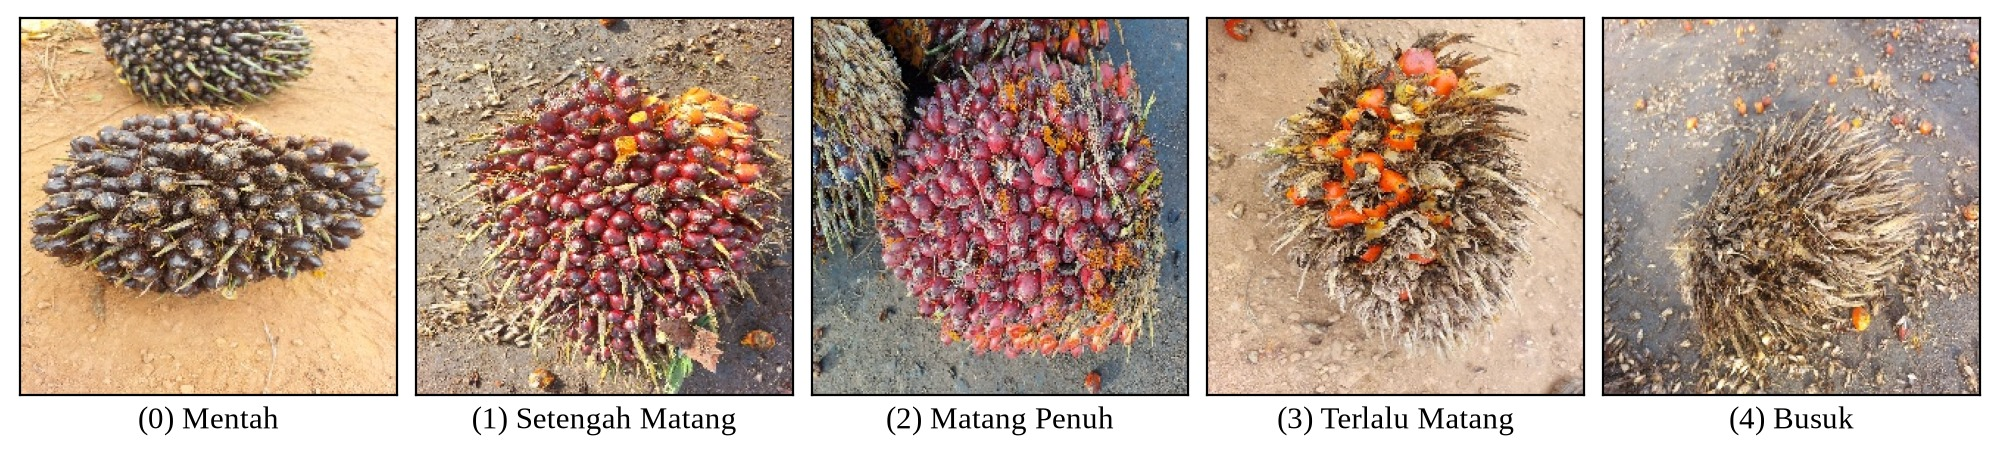
\includegraphics[width=\textwidth]{gambar/kelas_kematangan_bw.jpg}
  \caption{Contoh foto untuk setiap tingkat kematangan dalam dataset \cite{kamal2024}.}
  \label{fig:kelas}
\end{figure*}

\begin{figure*}[t]
  \centering
  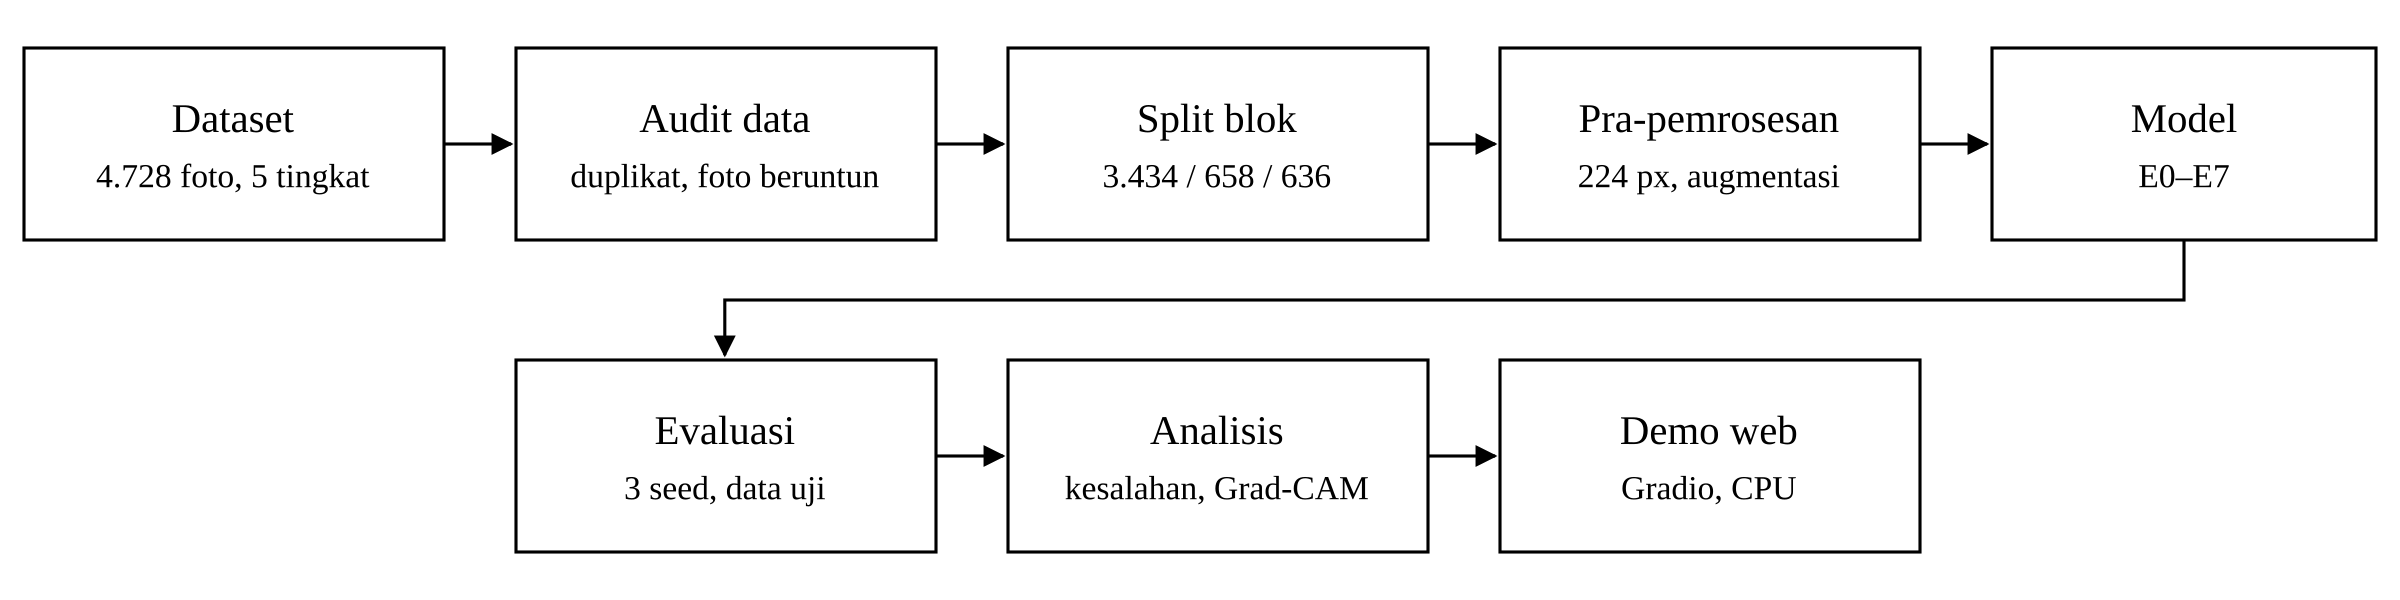
\includegraphics[width=0.88\textwidth]{gambar/alur_bw.png}
  \caption{Alur kerja proyek, dari dataset sampai demo web.}
  \label{fig:alur}
\end{figure*}

\section{2. Methodology / Metodologi}
Alur kerja proyek ditunjukkan pada Gambar~\ref{fig:alur}. Semua pengaturan disimpan dalam berkas konfigurasi YAML di repositori proyek agar eksperimen dapat diulang.

\subsection{A. Data Strategy / Strategi Data}
Dataset yang dipakai adalah \emph{An Ordinal Dataset for Ripeness Level Classification in Oil Palm Fruit Quality Grading} dari Mendeley Data \cite{kamal2024} dengan lisensi CC BY 4.0. Dataset ini berisi 4.728 foto JPG berukuran $256\times256$ piksel yang diambil di perkebunan Kalimantan Tengah dengan berbagai ponsel, pencahayaan, dan latar. Penyusun dataset juga menyediakan pembagian data resmi secara acak (Tabel~\ref{tab:data}).

\begin{table}[t]
  \centering
  \caption{Jumlah foto per kelas (latih / validasi / uji).}
  \label{tab:data}
  \footnotesize
  \setlength{\tabcolsep}{3pt}
  \begin{tabular}{|l|r|c|c|}
    \hline
    \textbf{Kelas} & \textbf{Total} & \textbf{Split resmi} & \textbf{Split blok} \\
    \hline
    Mentah          & 758   & 530 / 113 / 115   & 580 / 98 / 80     \\
    Setengah Matang & 1.405 & 982 / 210 / 213   & 1.025 / 180 / 200 \\
    Matang Penuh    & 1.489 & 1.042 / 222 / 225 & 1.069 / 220 / 200 \\
    Terlalu Matang  & 665   & 465 / 98 / 102    & 460 / 100 / 105   \\
    Busuk           & 411   & 287 / 61 / 63     & 300 / 60 / 51     \\
    \hline
    Total           & 4.728 & 3.306 / 704 / 718 & 3.434 / 658 / 636 \\
    \hline
  \end{tabular}
\end{table}

\textbf{Audit data.} Sebelum pelatihan, kami memeriksa duplikat dengan MD5 dan dHash, dan menemukan 1 pasang berkas identik serta 13 pasang foto yang hampir identik. Kami juga menemukan bahwa foto dengan nomor berkas berurutan sering memotret tandan yang sama dari sudut yang sedikit berbeda (Gambar~\ref{fig:bocor}). Dari 40 pasangan berurutan yang kami periksa secara manual, 62\% dari pasangan yang dapat diputuskan adalah tandan yang sama. Pada split resmi, 92\% foto uji memiliki foto bernomor $\pm1$ di data latih, sehingga model dapat diuji dengan tandan yang sudah pernah dilihatnya. Kebocoran data seperti ini membuat hasil terlihat lebih baik daripada sebenarnya \cite{kapoor2023}.

\begin{figure}[t]
  \centering
  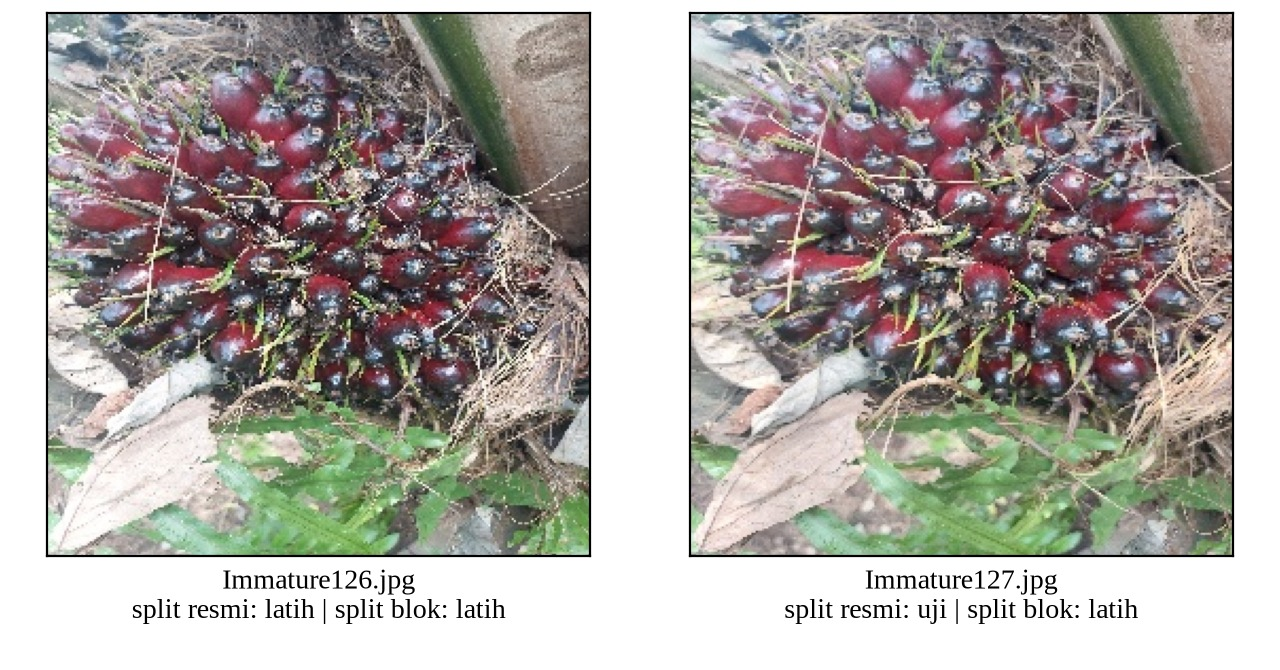
\includegraphics[width=\columnwidth]{gambar/contoh_kebocoran_bw.jpg}
  \caption{Dua foto tandan yang sama dengan nomor berkas berurutan.}
  \label{fig:bocor}
\end{figure}

\textbf{Split blok.} Untuk mengatasi kebocoran tersebut, nomor berkas setiap kelas dibagi menjadi blok berisi 20 foto berurutan. Blok-blok ini dibagi ke data latih, validasi, dan uji dengan \emph{StratifiedGroupKFold} (seed 42) sehingga satu blok selalu berada di bagian yang sama. Hasilnya 3.434 / 658 / 636 foto, dan hanya 8,3\% foto uji yang masih bertetangga dengan data latih, yaitu foto di batas blok. Split blok dipakai sebagai split utama, sedangkan split resmi hanya dipakai sebagai pembanding. Pembagian ini disimpan sebagai berkas CSV karena hasil \emph{StratifiedGroupKFold} dapat berbeda antarversi scikit-learn.

\textbf{Pra-pemrosesan dan augmentasi.} Saat pelatihan, foto dipotong acak dengan \emph{RandomResizedCrop} $224\times224$ (skala 0,6--1,0), dibalik secara horizontal dan vertikal, diputar $\pm15^\circ$, serta diubah kecerahan dan kontrasnya $\pm0{,}2$. \emph{Hue} dan saturasi tidak diubah karena warna adalah isyarat utama kematangan; pengaruhnya diuji terpisah (E4). Saat evaluasi, foto diubah ukurannya ke 256 lalu dipotong di tengah menjadi $224\times224$. Semua foto dinormalisasi dengan rerata dan simpangan baku ImageNet.

\textbf{Ketidakseimbangan kelas.} Kelas terbesar (Matang Penuh) berjumlah 3,6 kali kelas terkecil (Busuk). Karena itu kami memakai macro-F1 sebagai metrik utama dan untuk memilih checkpoint, melaporkan recall per kelas, dan menguji \emph{WeightedRandomSampler} yang menyeimbangkan kelas (E5).

\subsection{B. Model Architecture / Arsitektur Model}
\textbf{Baseline.} Ada dua baseline klasik: E0 selalu menebak kelas terbanyak, dan E1 memakai 40 fitur histogram warna HSV dengan regresi logistik. Baseline ketiga adalah E2, yaitu EfficientNet-B0 dengan \emph{cross-entropy}.

\textbf{Backbone.} Kami memakai EfficientNet-B0 \cite{tan2019} dengan bobot pra-latih ImageNet \cite{deng2009} dari torchvision. Lapisan klasifikasinya diganti dengan \emph{Dropout}(0,2) dan \emph{Linear}($1280 \rightarrow K$), sehingga model memiliki sekitar 4,0 juta parameter. Seluruh lapisan dilatih ulang (\emph{full fine-tuning}).

\textbf{Kepala CE dan CORN.} Kepala CE (E2) menghasilkan $K=5$ logit dan dilatih dengan \emph{cross-entropy}. Kepala CORN (E3) menghasilkan $K-1=4$ logit. Logit ke-$k$ memodelkan peluang bersyarat $P(y>k \mid y>k-1)$ dan dilatih dengan \emph{binary cross-entropy} hanya pada sampel dengan $y \geq k$ \cite{shi2023}. Peluang kumulatifnya dihitung sebagai
\begin{equation}
  P(y>k) = \prod_{j \leq k} \sigma(z_j),
\end{equation}
dan tingkat yang diprediksi adalah banyaknya $k$ dengan $P(y>k) > 0{,}5$. Kedua model memakai backbone, data, dan pengaturan pelatihan yang sama (Tabel~\ref{tab:latih}); yang berbeda hanya kepala dan loss-nya.

\begin{table}[t]
  \centering
  \caption{Pengaturan pelatihan.}
  \label{tab:latih}
  \footnotesize
  \begin{tabular}{|l|p{4.6cm}|}
    \hline
    \textbf{Parameter} & \textbf{Nilai} \\
    \hline
    Optimizer            & AdamW \cite{loshchilov2019}, lr $3\cdot10^{-4}$, \emph{weight decay} $10^{-2}$ \\
    Jadwal lr            & \emph{warmup} 1 epoch, lalu \emph{cosine decay} \\
    Epoch / batch        & maks. 25, \emph{early stopping} 7 epoch; batch 32 \\
    Pemilihan checkpoint & macro-F1 validasi terbaik \\
    Seed                 & 42, 43, 44 \\
    \hline
  \end{tabular}
\end{table}

\textbf{Eksperimen.} Tabel~\ref{tab:eksperimen} merangkum eksperimen yang dijalankan. Setiap perbandingan hanya mengubah satu faktor, dan setiap eksperimen CNN diulang dengan tiga seed.

\begin{table}[t]
  \centering
  \caption{Daftar eksperimen.}
  \label{tab:eksperimen}
  \footnotesize
  \begin{tabular}{|l|p{4.2cm}|l|}
    \hline
    \textbf{ID} & \textbf{Perlakuan} & \textbf{Split} \\
    \hline
    E0, E1 & kelas mayoritas; HSV + regresi logistik & blok, resmi \\
    E2     & EfficientNet-B0 + CE & blok \\
    E3     & EfficientNet-B0 + CORN & blok \\
    E4     & E3 + augmentasi \emph{hue} 0,1 dan saturasi 0,2 & blok \\
    E5     & E3 + sampler seimbang kelas & blok \\
    E6, E7 & E2 dan E3 & resmi \\
    \hline
  \end{tabular}
\end{table}

\textbf{Evaluasi.} Data uji hanya dievaluasi sekali per run, setelah checkpoint dipilih dari data validasi. Metrik yang dipakai adalah akurasi, macro-F1, recall per kelas, dan \emph{confusion matrix}, ditambah tiga metrik ordinal: MAE (rata-rata selisih tingkat), proporsi kesalahan berat (meleset $\geq 2$ tingkat), dan \emph{quadratic weighted kappa} \cite{cohen1968}. Hasil dilaporkan sebagai rerata $\pm$ simpangan baku dari tiga seed. Untuk analisis kesalahan, kami memakai Grad-CAM \cite{selvaraju2017} untuk melihat bagian foto yang paling memengaruhi prediksi.

\subsection{C. Deployment \& Environment / Lingkungan \& Penerapan}
Pelatihan dilakukan di Google Colab dengan GPU NVIDIA Tesla T4 (16~GB), PyTorch 2.11, dan CUDA 13.0. Satu run memakan waktu sekitar 7--15 menit, dengan total 18 run CNN. Baseline klasik, analisis kesalahan, dan demo dijalankan di laptop dengan CPU AMD Ryzen 5 5600.

Model dipakai melalui aplikasi web Gradio yang berjalan di laptop. Pengguna mengunggah foto lewat peramban. Server menjalankan pra-pemrosesan yang sama dengan data validasi, memuat checkpoint model ($\pm$16~MB), lalu menampilkan tingkat kematangan, peluang setiap tingkat, peta Grad-CAM, dan peringatan bila keyakinan model di bawah 0,9. Ambang ini dipilih dari data validasi. Waktu inferensi diukur dengan batch 1 dan 100 iterasi, dan hasilnya sekitar 12~ms per foto pada CPU. Sebagai cadangan bila antarmuka web bermasalah, prediksi juga dapat dijalankan melalui skrip baris perintah.

\begin{thebibliography}{99}
\small
\bibitem{pusdatin2024} Pusat Data dan Sistem Informasi Pertanian, \emph{Outlook Kelapa Sawit 2024}. Jakarta: Kementerian Pertanian RI, 2024.

\bibitem{woittiez2016} L.~S. Woittiez \emph{et al.}, \emph{Smallholder Oil Palm Handbook, Module 2: Harvesting, Grading, Transport}, 3rd ed. Wageningen University \& SNV, 2016.

\bibitem{alfatni2008} M.~S.~M. Alfatni \emph{et al.}, ``Oil palm fruit bunch grading system using red, green and blue digital number,'' \emph{Journal of Applied Sciences}, vol.~8, no.~8, pp.~1444--1452, 2008.

\bibitem{suharjito2021} Suharjito, G.~N. Elwirehardja, and J.~S. Prayoga, ``Oil palm fresh fruit bunch ripeness classification on mobile devices using deep learning approaches,'' \emph{Computers and Electronics in Agriculture}, vol.~188, 106359, 2021.

\bibitem{deng2009} J.~Deng \emph{et al.}, ``ImageNet: A large-scale hierarchical image database,'' in \emph{Proc. CVPR}, 2009, pp.~248--255.

\bibitem{kamal2024} I.~M. Kamal \emph{et al.}, ``An ordinal dataset for ripeness level classification in oil palm fruit quality grading,'' Mendeley Data, v1, 2024, doi: 10.17632/424y96m6sw.1.

\bibitem{shi2023} X.~Shi, W.~Cao, and S.~Raschka, ``Deep neural networks for rank-consistent ordinal regression based on conditional probabilities,'' \emph{Pattern Analysis and Applications}, vol.~26, no.~3, pp.~941--955, 2023.

\bibitem{kapoor2023} S.~Kapoor and A.~Narayanan, ``Leakage and the reproducibility crisis in machine-learning-based science,'' \emph{Patterns}, vol.~4, no.~9, 100804, 2023.

\bibitem{tan2019} M.~Tan and Q.~V. Le, ``EfficientNet: Rethinking model scaling for convolutional neural networks,'' in \emph{Proc. ICML}, 2019, pp.~6105--6114.

\bibitem{loshchilov2019} I.~Loshchilov and F.~Hutter, ``Decoupled weight decay regularization,'' in \emph{Proc. ICLR}, 2019.

\bibitem{cohen1968} J.~Cohen, ``Weighted kappa: Nominal scale agreement provision for scaled disagreement or partial credit,'' \emph{Psychological Bulletin}, vol.~70, no.~4, pp.~213--220, 1968.

\bibitem{selvaraju2017} R.~R. Selvaraju \emph{et al.}, ``Grad-CAM: Visual explanations from deep networks via gradient-based localization,'' in \emph{Proc. ICCV}, 2017, pp.~618--626.
\end{thebibliography}

\end{document}
